\documentclass[aspectratio=169,12pt,t]{beamer}

% --- Theme: Metropolis (modern, clean) ---
\usetheme[progressbar=frametitle,numbering=fraction,block=fill]{metropolis}

% --- Fira Sans font (install texlive-fonts-extra if missing) ---
\IfFileExists{FiraSans.sty}{\usepackage[sfdefault]{FiraSans}}{}

% --- Light background with warm accent ---
\definecolor{mDarkTeal}{RGB}{35,55,59}
\definecolor{mLightBrown}{RGB}{235,228,216}
\definecolor{mAccent}{RGB}{140,70,20}

\setbeamercolor{normal text}{fg=mDarkTeal,bg=white}
\setbeamercolor{alerted text}{fg=mAccent}
\setbeamercolor{frametitle}{bg=mDarkTeal,fg=white}
\setbeamercolor{progress bar}{fg=mAccent,bg=mLightBrown}
\setbeamercolor{title separator}{fg=mAccent}
\setbeamercolor{progress bar in head/foot}{fg=mAccent,bg=mLightBrown}
\setbeamercolor{progress bar in section page}{fg=mAccent,bg=mLightBrown}

% --- Packages ---
\usepackage[utf8]{inputenc}
\usepackage{amsmath,amssymb,amsthm}
\usepackage{mathrsfs}
\usepackage{tikz}
\usetikzlibrary{arrows.meta,positioning,calc,decorations.pathreplacing,shapes,patterns}
\usepackage{pgfplots}
\pgfplotsset{compat=1.18}

% --- TikZ diagram styles (shared across the series) ---
\tikzset{
  axisln/.style={-{Stealth[length=2.6mm]}, line width=0.8pt, gray!75},
  curveln/.style={line width=1.6pt, line cap=round, line join=round},
  projln/.style={dash pattern=on 2.6pt off 2pt, line width=0.7pt},
  guide/.style={-{Stealth[length=2.6mm,width=2.2mm]}, line width=1.1pt},
  vec/.style={-{Stealth[length=3mm,width=2.4mm]}, line width=1.4pt},
}
% point marker with a white halo: \dotpt{color}{(coord)}
\newcommand{\dotpt}[2]{%
  \fill[white] #2 circle (3.6pt);
  \fill[#1] #2 circle (2.4pt);
}
% open point marker: \opendotpt{color}{(coord)}
\newcommand{\opendotpt}[2]{%
  \fill[white] #2 circle (3.6pt);
  \draw[#1, line width=1pt] #2 circle (2.4pt);
}

% --- Semi-transparent white highlight for text on top of background images ---
\usepackage[most]{tcolorbox}

% Inline highlight: \hl{short text}
\newtcbox{\hl}{%
  nobeforeafter, tcbox raise base,
  colback=white, opacityback=0.6,
  colframe=white, opacityframe=0,
  sharp corners, boxsep=2pt, left=3pt, right=3pt, top=2pt, bottom=2pt%
}

% Block highlight: \begin{hlbox} ... \end{hlbox}  (multi-line, paragraphs, itemize)
% Optional argument accepts any tcolorbox key, e.g. [width=0.6\linewidth]
\newtcolorbox{hlbox}[1][]{%
  enhanced, breakable,
  colback=white, opacityback=0.6,
  colframe=white, opacityframe=0,
  boxsep=3pt, left=6pt, right=6pt, top=4pt, bottom=4pt,
  sharp corners,
  {#1}%
}

% --- Custom colors for content types ---
\definecolor{defcolor}{RGB}{25,85,120}
\definecolor{thmcolor}{RGB}{140,35,35}
\definecolor{proofcolor}{RGB}{35,100,50}
\definecolor{excolor}{RGB}{140,75,10}
\definecolor{remcolor}{RGB}{90,90,90}

% --- Beamer blocks for mathematical content types (semi-transparent) ---
\tcbset{hlblockbase/.style={
  enhanced, breakable,
  coltitle=white, fonttitle=\bfseries,
  opacitybacktitle=0.8, opacityback=0.6,
  opacityframe=0,
  sharp corners,
  boxsep=1pt, left=5pt, right=5pt, top=2pt, bottom=2pt,
  toptitle=1pt, bottomtitle=1pt
}}

\newtcolorbox{defblock}[1]{hlblockbase, title={#1},
  colbacktitle=defcolor, colback=defcolor!15, colframe=defcolor}
\newtcolorbox{thmblock}[1]{hlblockbase, title={#1},
  colbacktitle=thmcolor, colback=thmcolor!15, colframe=thmcolor}
\newtcolorbox{proofblock}[1]{hlblockbase, title={#1},
  colbacktitle=proofcolor, colback=proofcolor!15, colframe=proofcolor}
\newtcolorbox{exblock}[1]{hlblockbase, title={#1},
  colbacktitle=excolor, colback=excolor!15, colframe=excolor}
\newtcolorbox{remblock}[1]{hlblockbase, title={#1},
  colbacktitle=remcolor, colback=remcolor!15, colframe=remcolor}

% --- Metadata ---
\title{Chapter 6: The Riemann--Stieltjes Integral}
\subtitle{Section: Integration of Vector-Valued Functions}
\author{Based on Walter Rudin's \emph{Principles of Mathematical Analysis}}
\date{}

\begin{document}

{
\usebackgroundtemplate{%
  
\includegraphics[width=\paperwidth,height=\paperheight,keepaspectratio=false]{chapter_06_bg_00.png}%
}
\begin{frame}[plain]
  \titlepage

  \note{
    Welcome to Chapter 6, Section 4: Integration of Vector-Valued
    Functions. So far in this chapter every function we integrated
    was real valued. In this short episode we extend the
    Riemann-Stieltjes integral to functions whose values are vectors
    in "k" dimensional space. The definition is exactly what you
    would guess: integrate one coordinate at a time. Most of the
    theory then carries over for free, including the Fundamental
    Theorem of Calculus. But one result, the inequality that bounds
    the absolute value of an integral by the integral of the
    absolute value, needs a genuinely new idea in its proof, and
    that idea is the Schwarz inequality from Chapter 1. Along the
    way we will see a beautiful geometric meaning: the straight line
    displacement of a moving point can never exceed the distance it
    actually traveled. Let's begin.
  }
\end{frame}
}

{
\usebackgroundtemplate{%
  
\includegraphics[width=\paperwidth,height=\paperheight,keepaspectratio=false]{chapter_06_bg_01.png}%
}
\begin{frame}[c]{Outline}
  \begin{center}
    \tableofcontents
  \end{center}

  \note{
    Here is the plan for this episode. We start with some motivation:
    why vector valued integrals are natural, and what we should
    expect to survive the passage from numbers to vectors. Then
    comes Definition 6.23, the componentwise integral, together with
    a tour of the results that carry over immediately. Next is
    Theorem 6.24, the vector form of the Fundamental Theorem of
    Calculus, with a worked example. The heart of the episode is
    Theorem 6.25, the triangle inequality for vector integrals, whose
    proof uses the Schwarz inequality in a clever way. We close with
    a summary and a preview of the next section on rectifiable
    curves.
  }
\end{frame}

\section{Motivation}

% --- Build 1/3 ---
\begin{frame}{From Numbers to Vectors}
  \begin{hlbox}
  \begin{itemize}
    \item Chapter 5, Section 7: we \alert{differentiated} maps
      $\mathbf{f} : [a, b] \to R^k$ \emph{componentwise}
  \end{itemize}
  \end{hlbox}

  \note{
    Let's recall where we have been. At the end of Chapter 5 we
    studied vector valued functions, maps from an interval into "k"
    dimensional space. We differentiated them one coordinate at a
    time: the derivative of "f" is the vector whose components are
    the derivatives of the components of "f". Geometrically, if "f"
    of "t" is the position of a moving point at time "t", then the
    derivative is its velocity vector. This componentwise philosophy
    is going to guide us again today.
  }
\end{frame}

% --- Build 2/3 ---
\begin{frame}{From Numbers to Vectors}
  \begin{hlbox}
  \begin{itemize}
    \item Chapter 5, Section 7: we \alert{differentiated} maps
      $\mathbf{f} : [a, b] \to R^k$ \emph{componentwise}
    \item Natural next step: \alert{integrate} them componentwise too
  \end{itemize}
  \end{hlbox}

  \note{
    The natural next step is to integrate vector valued functions,
    and again the obvious thing to do is to integrate one coordinate
    at a time. The integral of "f" will be a point in "k" dimensional
    space, whose coordinate number "j" is the integral of component number "j". If "f" is a velocity, its integral should be the net
    displacement, and that is exactly what this definition delivers.
    So the definition is easy. The real question is a different one.
  }
\end{frame}

% --- Build 3/3 ---
\begin{frame}{From Numbers to Vectors}
  \begin{hlbox}
  \begin{itemize}
    \item Chapter 5, Section 7: we \alert{differentiated} maps
      $\mathbf{f} : [a, b] \to R^k$ \emph{componentwise}
    \item Natural next step: \alert{integrate} them componentwise too
    \item The real question: \emph{which theorems survive?}
      \begin{itemize}
        \item anything stated coordinate by coordinate --- \alert{for free}
        \item anything using \emph{order} or \emph{absolute values} ---
          \alert{needs care}
      \end{itemize}
  \end{itemize}
  \end{hlbox}

  \note{
    The real question is which of the theorems from the earlier
    sections survive the passage to vector values. There is a simple
    rule of thumb. Any statement that can be checked one coordinate
    at a time, such as linearity, splitting the interval, or the
    Fundamental Theorem of Calculus, carries over for free: we just
    apply the real valued result to each component. But anything
    that uses the order of the real line, or absolute values, needs
    care, because vectors are not ordered, and the length of a
    vector is not computed coordinate by coordinate. That is where
    the interesting mathematics of this section lives.
  }
\end{frame}

\begin{frame}{The Picture to Keep in Mind}
  \begin{center}
  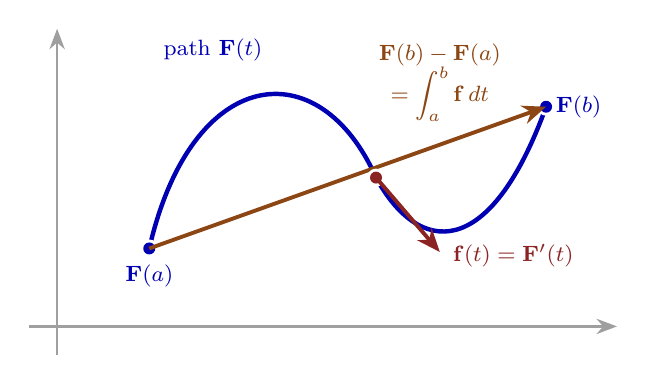
\begin{tikzpicture}[scale=0.9]
    \draw[axisln] (-0.9,-0.5) -- (7.4,-0.5);
    \draw[axisln] (-0.5,-0.9) -- (-0.5,3.7);
    % curve F(t) from A to B
    \draw[curveln, blue!70!black]
      (0.8,0.6) .. controls (1.4,3.2) and (3.2,3.4) .. (4.0,1.6)
      .. controls (4.6,0.5) and (5.6,0.4) .. (6.4,2.6);
    \dotpt{blue!70!black}{(0.8,0.6)}
    \dotpt{blue!70!black}{(6.4,2.6)}
    \node[blue!70!black, below] at (0.8,0.5) {\footnotesize $\mathbf{F}(a)$};
    \node[blue!70!black, right] at (6.4,2.6) {\footnotesize $\mathbf{F}(b)$};
    \node[blue!70!black] at (1.7,3.4) {\footnotesize path $\mathbf{F}(t)$};
    % displacement vector
    \draw[vec, mAccent] (0.8,0.6) -- (6.4,2.6);
    \node[mAccent, anchor=south, align=center] at (4.9,2.25)
      {\footnotesize $\mathbf{F}(b)-\mathbf{F}(a)$\\[-1pt] \footnotesize $\displaystyle = \int_a^b \mathbf{f}\,dt$};
    % velocity vector at a point
    \dotpt{thmcolor}{(4.0,1.6)}
    \draw[vec, thmcolor] (4.0,1.6) -- (4.9,0.55);
    \node[thmcolor, right] at (4.95,0.5) {\footnotesize $\mathbf{f}(t) = \mathbf{F}'(t)$};
  \end{tikzpicture}
  \end{center}

  \vspace{-0.3em}
  \begin{center}
  \hl{\textbf{Displacement} $\left|\int_a^b \mathbf{f}\,dt\right|$ \;versus\;
  \textbf{distance traveled} $\int_a^b |\mathbf{f}|\,dt$}
  \end{center}

  \note{
    Here is the picture that organizes the whole section. The blue
    curve is the path of a moving point capital "F" of "t" in the plane,
    starting at the lower left point capital "F" of "a" and ending at the
    upper right point capital "F" of "b". The red arrow is the velocity
    vector at one intermediate moment, the derivative of capital "F", which
    we call lowercase "f". The orange arrow is the straight line
    displacement from start to finish, and its label records what the
    vector form of the Fundamental Theorem will tell us: this
    displacement, capital "F" of "b" minus capital "F" of "a", is exactly the
    integral of the velocity "f". Now compare two numbers: the length of the orange
    arrow, which is the absolute value of the integral of "f", and
    the length of the blue path, which is the integral of the
    absolute value of "f". Clearly the straight line is shorter.
    That inequality is Theorem 6.25, and it is the main goal of this
    episode.
  }
\end{frame}

% --- Build 1/3 ---
\begin{frame}{What We Will Prove}
  \begin{hlbox}
  \begin{itemize}
    \item \textbf{Definition 6.23:} $\displaystyle \int_a^b \mathbf{f}\,d\alpha
      = \Big(\int_a^b f_1\,d\alpha, \dots, \int_a^b f_k\,d\alpha\Big)$
  \end{itemize}
  \end{hlbox}

  \note{
    Let's preview the three items of this section. First,
    Definition 6.23 makes the componentwise idea official: the
    integral of a vector valued function with respect to alpha is
    the vector of the integrals of its components. We will also list
    which earlier theorems come along for free.
  }
\end{frame}

% --- Build 2/3 ---
\begin{frame}{What We Will Prove}
  \begin{hlbox}
  \begin{itemize}
    \item \textbf{Definition 6.23:} $\displaystyle \int_a^b \mathbf{f}\,d\alpha
      = \Big(\int_a^b f_1\,d\alpha, \dots, \int_a^b f_k\,d\alpha\Big)$
    \item \textbf{Theorem 6.24 (FTC):} $\mathbf{F}' = \mathbf{f} \in \mathscr{R}$
      $\;\Longrightarrow\;$ $\displaystyle \int_a^b \mathbf{f}\,dt = \mathbf{F}(b) - \mathbf{F}(a)$
  \end{itemize}
  \end{hlbox}

  \note{
    Second, Theorem 6.24, the Fundamental Theorem of Calculus for
    vector valued functions. If capital "F" has derivative "f", and "f" is
    integrable, then the integral of "f" is capital "F" of "b" minus capital "F" of
    "a". This is the displacement statement from the picture, and
    its proof is one line: apply the real Fundamental Theorem to each
    coordinate.
  }
\end{frame}

% --- Build 3/3 ---
\begin{frame}{What We Will Prove}
  \begin{hlbox}
  \begin{itemize}
    \item \textbf{Definition 6.23:} $\displaystyle \int_a^b \mathbf{f}\,d\alpha
      = \Big(\int_a^b f_1\,d\alpha, \dots, \int_a^b f_k\,d\alpha\Big)$
    \item \textbf{Theorem 6.24 (FTC):} $\mathbf{F}' = \mathbf{f} \in \mathscr{R}$
      $\;\Longrightarrow\;$ $\displaystyle \int_a^b \mathbf{f}\,dt = \mathbf{F}(b) - \mathbf{F}(a)$
    \item \textbf{Theorem 6.25:} $\mathbf{f} \in \mathscr{R}(\alpha)$
      $\;\Longrightarrow\;$ $|\mathbf{f}| \in \mathscr{R}(\alpha)$ and
      $\displaystyle \Big|\int_a^b \mathbf{f}\,d\alpha\Big| \leq \int_a^b |\mathbf{f}|\,d\alpha$
      \\[2pt] \hspace{1.2em} \emph{new ingredient:} the \alert{Schwarz inequality}
  \end{itemize}
  \end{hlbox}

  \note{
    Third, and this is the centerpiece, Theorem 6.25. If "f" is
    integrable, then so is its length, the function absolute value of
    "f", and the absolute value of the integral is at most the
    integral of the absolute value. The real valued version of this
    was part "b" of Theorem 6.13, and its proof used a sign trick
    that has no analogue for vectors. The new ingredient is the
    Schwarz inequality from Chapter 1, used in a way that is worth
    remembering. Let's start with the definition.
  }
\end{frame}
}

{
\usebackgroundtemplate{%
  
\includegraphics[width=\paperwidth,height=\paperheight,keepaspectratio=false]{chapter_06_bg_02.png}%
}
\section{Integrating Componentwise}

% --- Build 1/2 ---
\begin{frame}{Definition 6.23: Vector-Valued Integrals}
  \begin{defblock}{Definition 6.23}
    Let $f_1, \dots, f_k$ be real functions on $[a, b]$, and let
    $\mathbf{f} = (f_1, \dots, f_k)$ be the corresponding mapping of
    $[a, b]$ into $R^k$. If $\alpha$ increases monotonically on $[a, b]$,
    to say that $\mathbf{f} \in \mathscr{R}(\alpha)$ means that
    $f_j \in \mathscr{R}(\alpha)$ for $j = 1, \dots, k$.
  \end{defblock}

  \note{
    Here is Definition 6.23. We start with "k" real functions "f"
    sub 1 through "f" sub "k" on the interval, and we bundle them
    into a single map "f" from the interval into "k" dimensional
    space; coordinate number "j" of "f" of "t" is "f" sub "j" of
    "t". Let alpha be a monotonically increasing integrator, as
    usual. The first part of the definition says what integrability
    means for "f": we say that "f" is integrable with respect to
    alpha if every one of its components is integrable with respect
    to alpha, in the sense of Definition 6.2. Nothing new happens
    here; we simply require the real valued condition "k" times.
  }
\end{frame}

% --- Build 2/2 ---
\begin{frame}{Definition 6.23: Vector-Valued Integrals}
  \begin{defblock}{Definition 6.23}
    Let $f_1, \dots, f_k$ be real functions on $[a, b]$, and let
    $\mathbf{f} = (f_1, \dots, f_k)$ be the corresponding mapping of
    $[a, b]$ into $R^k$. If $\alpha$ increases monotonically on $[a, b]$,
    to say that $\mathbf{f} \in \mathscr{R}(\alpha)$ means that
    $f_j \in \mathscr{R}(\alpha)$ for $j = 1, \dots, k$.
    If this is the case, we define
    \[
      \int_a^b \mathbf{f}\,d\alpha
      = \left(\int_a^b f_1\,d\alpha, \dots, \int_a^b f_k\,d\alpha\right).
    \]
  \end{defblock}

  \vspace{0.3em}
  \hl{$\int \mathbf{f}\,d\alpha$ is the \alert{point in $R^k$} whose $j$th
  coordinate is $\int f_j\,d\alpha$.}

  \note{
    When "f" is integrable in this sense, we define its integral to
    be the vector whose coordinate number "j" is the integral of "f" sub
    "j" with respect to alpha. In other words, the integral of a
    vector valued function is a point in "k" dimensional space,
    obtained by integrating one coordinate at a time. Notice that
    the integrator alpha is still a real valued increasing function;
    only the integrand has become vector valued. Let's look at a
    picture of what this definition does in the plane.
  }
\end{frame}

\begin{frame}{The Definition in a Picture ($k = 2$)}
  \begin{center}
  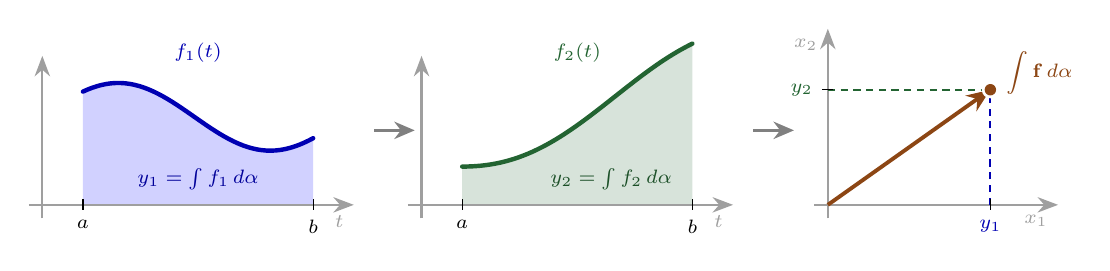
\begin{tikzpicture}[scale=0.86]
    % --- left: component f_1 ---
    \begin{scope}
      \fill[blue!18] plot[domain=0.6:4.0, samples=50]
        (\x, {1.3 + 0.5*sin(deg(1.4*\x))}) -- (4.0,0) -- (0.6,0) -- cycle;
      \draw[axisln] (-0.2,0) -- (4.6,0) node[below left]{\scriptsize $t$};
      \draw[axisln] (0,-0.2) -- (0,2.2);
      \draw[curveln, blue!70!black, domain=0.6:4.0, samples=50]
        plot (\x, {1.3 + 0.5*sin(deg(1.4*\x))});
      \draw (0.6,0.08) -- (0.6,-0.08) node[below]{\scriptsize $a$};
      \draw (4.0,0.08) -- (4.0,-0.08) node[below]{\scriptsize $b$};
      \node[blue!70!black] at (2.3,2.25) {\scriptsize $f_1(t)$};
      \node[blue!60!black] at (2.3,0.38) {\scriptsize $y_1 = \int f_1\,d\alpha$};
    \end{scope}
    % --- middle: component f_2 ---
    \begin{scope}[xshift=5.6cm]
      \fill[proofcolor!18] plot[domain=0.6:4.0, samples=50]
        (\x, {0.6 + 0.35*\x - 0.4*sin(deg(1.1*\x))}) -- (4.0,0) -- (0.6,0) -- cycle;
      \draw[axisln] (-0.2,0) -- (4.6,0) node[below left]{\scriptsize $t$};
      \draw[axisln] (0,-0.2) -- (0,2.2);
      \draw[curveln, proofcolor, domain=0.6:4.0, samples=50]
        plot (\x, {0.6 + 0.35*\x - 0.4*sin(deg(1.1*\x))});
      \draw (0.6,0.08) -- (0.6,-0.08) node[below]{\scriptsize $a$};
      \draw (4.0,0.08) -- (4.0,-0.08) node[below]{\scriptsize $b$};
      \node[proofcolor] at (2.3,2.25) {\scriptsize $f_2(t)$};
      \node[proofcolor!80!black] at (2.8,0.38) {\scriptsize $y_2 = \int f_2\,d\alpha$};
    \end{scope}
    % --- right: the resulting point in R^2 ---
    \begin{scope}[xshift=11.6cm]
      \draw[axisln] (-0.2,0) -- (3.4,0) node[below left]{\scriptsize $x_1$};
      \draw[axisln] (0,-0.2) -- (0,2.6) node[below left]{\scriptsize $x_2$};
      \draw[projln, blue!70!black] (2.4,0) -- (2.4,1.7);
      \draw[projln, proofcolor] (0,1.7) -- (2.4,1.7);
      \draw (2.4,0.08) -- (2.4,-0.08) node[below, blue!70!black]{\scriptsize $y_1$};
      \draw (0.08,1.7) -- (-0.08,1.7) node[left, proofcolor]{\scriptsize $y_2$};
      \draw[vec, mAccent] (0,0) -- (2.4,1.7);
      \dotpt{mAccent}{(2.4,1.7)}
      \node[mAccent, right] at (2.5,1.95) {\scriptsize $\displaystyle\int \mathbf{f}\,d\alpha$};
    \end{scope}
    % arrows joining panels
    \draw[guide, gray] (4.9,1.1) -- (5.5,1.1);
    \draw[guide, gray] (10.5,1.1) -- (11.1,1.1);
  \end{tikzpicture}
  \end{center}

  \vspace{-0.3em}
  \begin{hlbox}
  \textbf{Recipe:} integrate each component separately, then assemble
  the results into one point of $R^k$.
  \end{hlbox}

  \note{
    This picture shows the definition at work in the plane. On the
    left, the blue curve is the graph of the first component "f" sub
    1, and the shaded area is its integral, a real number "y" sub 1.
    In the middle, the green curve is the second component "f" sub
    2, and its shaded integral is another real number "y" sub 2. On
    the right we assemble the two numbers into one point: "y" sub 1
    is the horizontal coordinate, "y" sub 2 is the vertical
    coordinate, and the orange arrow points to the resulting vector,
    the integral of "f". That is the whole recipe: integrate each
    component separately, then put the answers together. With the
    definition understood, let's see what we get for free.
  }
\end{frame}

% --- Build 1/3 ---
\begin{frame}{What Carries Over for Free}
  \begin{hlbox}
  \textbf{Apply the real-valued result to each coordinate:}
  \begin{itemize}
    \item \textbf{Theorem 6.12(a):} \emph{linearity}:
      $\int (\mathbf{f} + \mathbf{g})\,d\alpha = \int \mathbf{f}\,d\alpha + \int \mathbf{g}\,d\alpha$,
      \quad $\int c\mathbf{f}\,d\alpha = c \int \mathbf{f}\,d\alpha$
  \end{itemize}
  \end{hlbox}

  \note{
    Since the vector integral is built coordinate by coordinate, any
    theorem about real integrals that holds coordinate by coordinate
    transfers immediately. The book lists them, and we go through
    the list. First, linearity, part "a" of Theorem 6.12: the
    integral of a sum of vector functions is the sum of the
    integrals, and constants pull out. Why? Because each coordinate
    of the sum is the sum of the coordinates, and the real valued
    theorem applies to each of them.
  }
\end{frame}

% --- Build 2/3 ---
\begin{frame}{What Carries Over for Free}
  \begin{hlbox}
  \textbf{Apply the real-valued result to each coordinate:}
  \begin{itemize}
    \item \textbf{Theorem 6.12(a):} \emph{linearity}:
      $\int (\mathbf{f} + \mathbf{g})\,d\alpha = \int \mathbf{f}\,d\alpha + \int \mathbf{g}\,d\alpha$,
      \quad $\int c\mathbf{f}\,d\alpha = c \int \mathbf{f}\,d\alpha$
    \item \textbf{Theorem 6.12(c):} \emph{splitting the interval}:
      $\int_a^c \mathbf{f}\,d\alpha + \int_c^b \mathbf{f}\,d\alpha = \int_a^b \mathbf{f}\,d\alpha$
    \item \textbf{Theorem 6.12(e):} \emph{linearity in $\alpha$}:
      $\int \mathbf{f}\,d(\alpha_1 + \alpha_2) = \int \mathbf{f}\,d\alpha_1 + \int \mathbf{f}\,d\alpha_2$
  \end{itemize}
  \end{hlbox}

  \note{
    Next, part "c" of Theorem 6.12: the integral over the whole
    interval is the sum of the integrals over the two pieces on
    either side of a point "c". And part "e", linearity in the
    integrator: integrating against a sum of two increasing functions
    gives the sum of the two integrals, and a positive constant
    multiplying alpha pulls out. Again, both statements are equalities
    between vectors, and two vectors are equal exactly when all
    their coordinates agree, so the real valued theorem does all the
    work. Notice which parts of Theorem 6.12 are missing from this
    list: part "b", monotonicity, and part "d", the absolute value
    bound. Both involve order or absolute values. We will come back
    to that.
  }
\end{frame}

% --- Build 3/3 ---
\begin{frame}{What Carries Over for Free}
  \begin{hlbox}
  \textbf{Apply the real-valued result to each coordinate:}
  \begin{itemize}
    \item \textbf{Theorem 6.12(a):} \emph{linearity}:
      $\int (\mathbf{f} + \mathbf{g})\,d\alpha = \int \mathbf{f}\,d\alpha + \int \mathbf{g}\,d\alpha$,
      \quad $\int c\mathbf{f}\,d\alpha = c \int \mathbf{f}\,d\alpha$
    \item \textbf{Theorem 6.12(c):} \emph{splitting the interval}:
      $\int_a^c \mathbf{f}\,d\alpha + \int_c^b \mathbf{f}\,d\alpha = \int_a^b \mathbf{f}\,d\alpha$
    \item \textbf{Theorem 6.12(e):} \emph{linearity in $\alpha$}:
      $\int \mathbf{f}\,d(\alpha_1 + \alpha_2) = \int \mathbf{f}\,d\alpha_1 + \int \mathbf{f}\,d\alpha_2$
    \item \textbf{Theorems 6.17, 6.20, 6.21:} reduction to the Riemann
      integral $\int \mathbf{f}\,d\alpha = \int \mathbf{f}\alpha'\,dx$;
      continuity and differentiability of $\mathbf{F}(x) = \int_a^x \mathbf{f}\,dt$;
      the \alert{Fundamental Theorem}
  \end{itemize}
  \end{hlbox}

  \note{
    Finally, three results from the later sections also carry over.
    Theorem 6.17, which converts a Stieltjes integral into an
    ordinary Riemann integral when alpha has an integrable
    derivative. Theorem 6.20, which says that the integral as a
    function of its upper limit is continuous, and differentiable
    with derivative "f" at the points where "f" is continuous. And
    Theorem 6.21, the Fundamental Theorem of Calculus. Each of these
    is a statement about individual coordinates, so each survives. To
    illustrate the pattern, the book states the vector version of the
    Fundamental Theorem explicitly, and that is Theorem 6.24.
  }
\end{frame}
}

{
\usebackgroundtemplate{%
  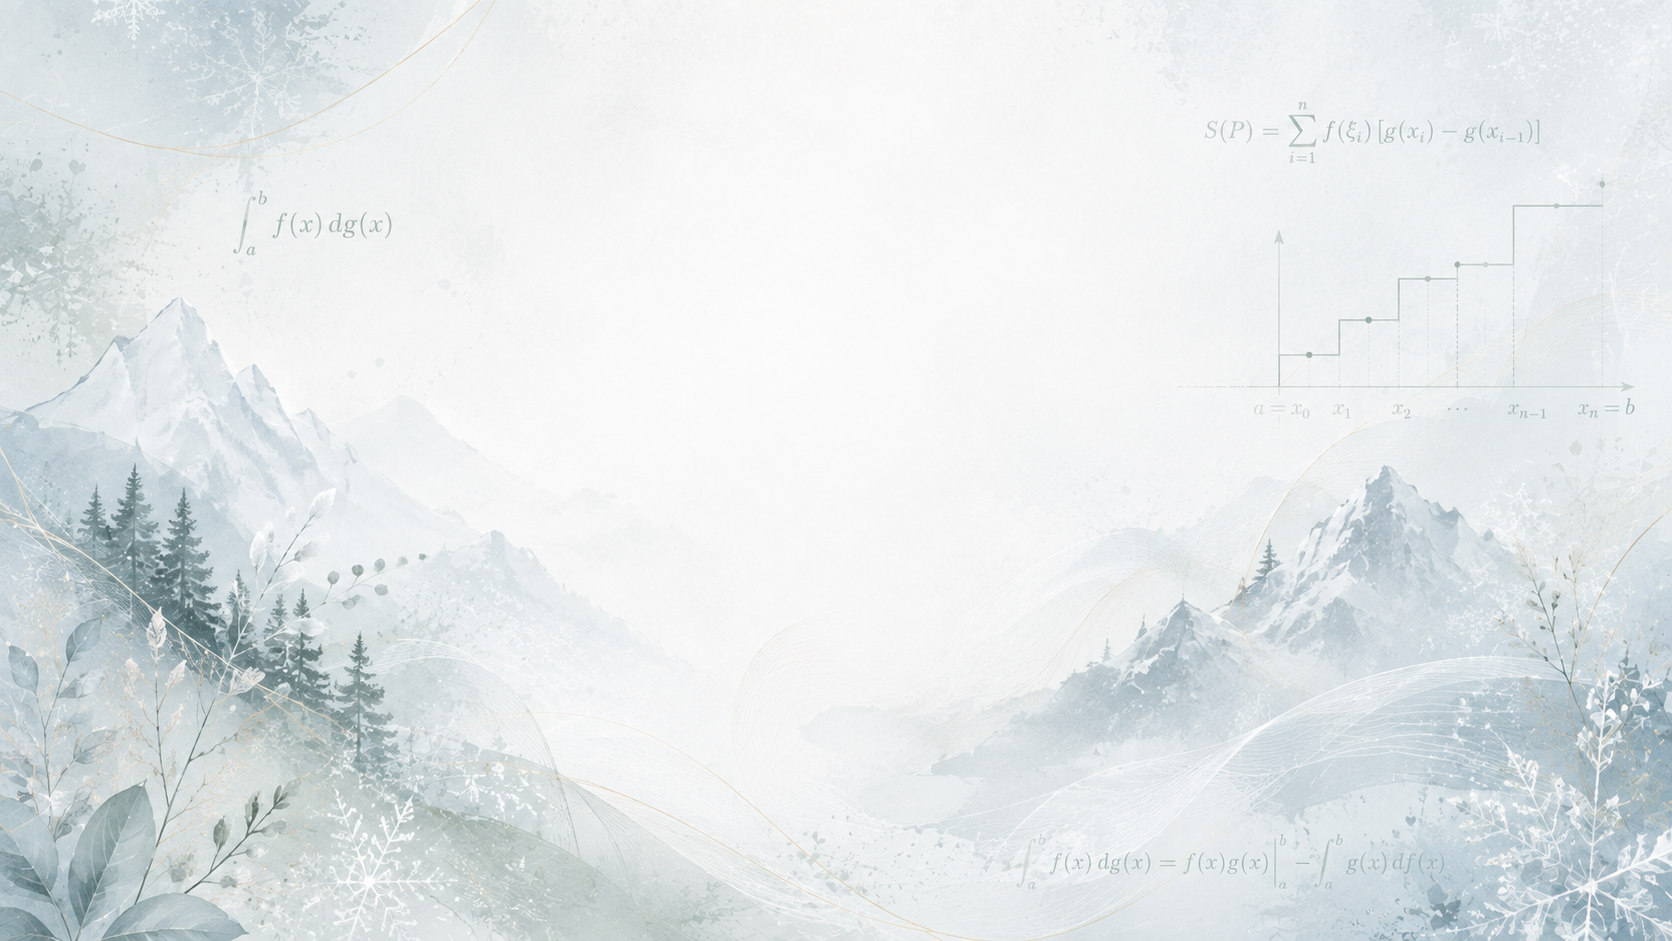
\includegraphics[width=\paperwidth,height=\paperheight,keepaspectratio=false]{chapter_06_bg_03.png}%
}
\section{The Fundamental Theorem, Vector Version}

\begin{frame}{Theorem 6.24: The Fundamental Theorem of Calculus}
  \begin{thmblock}{Theorem 6.24}
    If $\mathbf{f}$ and $\mathbf{F}$ map $[a, b]$ into $R^k$, if
    $\mathbf{f} \in \mathscr{R}$ on $[a, b]$, and if $\mathbf{F}' = \mathbf{f}$, then
    \[
      \int_a^b \mathbf{f}(t)\,dt = \mathbf{F}(b) - \mathbf{F}(a).
    \]
  \end{thmblock}

  \vspace{0.4em}
  \begin{hlbox}
  \textbf{Interpretation:} $\mathbf{f}$ = velocity, $\mathbf{F}$ = position.
  Integrating the velocity gives the \alert{net displacement}.
  \end{hlbox}

  \note{
    Here is Theorem 6.24. Two functions appear: lowercase "f" and
    capital "F". Suppose both map the interval into "k" dimensional space, "f" is Riemann integrable, and capital "F"
    is an antiderivative of "f", meaning that the derivative of capital "F",
    in the sense of Chapter 5 Section 7, is "f". Then the integral
    of "f" over the interval equals capital "F" of "b" minus capital "F" of "a", a
    difference of two vectors. In the physical picture, "f" is the
    velocity of a moving point and capital "F" is its position. The theorem
    says that integrating the velocity over a time interval gives
    the net displacement, the vector from the starting position to
    the final position. Let's see why the proof is immediate.
  }
\end{frame}

% --- Build 1/3 ---
\begin{frame}{Proof of Theorem 6.24: Coordinate by Coordinate}
  \begin{proofblock}{Step 1: Unpack the hypothesis}
    Write $\mathbf{f} = (f_1, \dots, f_k)$ and $\mathbf{F} = (F_1, \dots, F_k)$.
    By Chapter 5 (differentiation is componentwise),
    $\;\mathbf{F}' = \mathbf{f} \iff F_j' = f_j$ for $j = 1, \dots, k$.
  \end{proofblock}

  \note{
    Step 1: we unpack the hypothesis. Write "f" and capital "F" in
    coordinates. In Chapter 5, Section 7, we saw that a vector valued
    function is differentiable exactly when each of its components is
    differentiable, and that its derivative is the vector of the
    component derivatives. So the single vector equation capital "F" prime
    equals "f" is the same as "k" scalar equations: capital "F" sub "j"
    prime equals "f" sub "j" for every index "j". Also, by
    Definition 6.23, "f" integrable means each "f" sub "j" is
    integrable.
  }
\end{frame}

% --- Build 2/3 ---
\begin{frame}{Proof of Theorem 6.24: Coordinate by Coordinate}
  \begin{proofblock}{Step 1: Unpack the hypothesis}
    Write $\mathbf{f} = (f_1, \dots, f_k)$ and $\mathbf{F} = (F_1, \dots, F_k)$.
    By Chapter 5 (differentiation is componentwise),
    $\;\mathbf{F}' = \mathbf{f} \iff F_j' = f_j$ for $j = 1, \dots, k$.
  \end{proofblock}

  \begin{proofblock}{Step 2: Apply the real FTC (Theorem 6.21) to each coordinate}
    Each $f_j \in \mathscr{R}$ and $F_j' = f_j$, so
    $\;\displaystyle\int_a^b f_j(t)\,dt = F_j(b) - F_j(a)$ for $j = 1, \dots, k$.
  \end{proofblock}

  \note{
    Step 2: for each fixed "j", the real valued function "f" sub "j"
    is integrable and has the antiderivative capital "F" sub "j". These are
    exactly the hypotheses of Theorem 6.21, the Fundamental Theorem
    of Calculus from the previous episode. It gives us that the
    integral of "f" sub "j" equals capital "F" sub "j" of "b" minus capital "F" sub
    "j" of "a". We get one such equation for every coordinate.
  }
\end{frame}

% --- Build 3/3 ---
\begin{frame}{Proof of Theorem 6.24: Coordinate by Coordinate}
  \begin{proofblock}{Step 1: Unpack the hypothesis}
    Write $\mathbf{f} = (f_1, \dots, f_k)$ and $\mathbf{F} = (F_1, \dots, F_k)$.
    By Chapter 5 (differentiation is componentwise),
    $\;\mathbf{F}' = \mathbf{f} \iff F_j' = f_j$ for $j = 1, \dots, k$.
  \end{proofblock}

  \begin{proofblock}{Step 2: Apply the real FTC (Theorem 6.21) to each coordinate}
    Each $f_j \in \mathscr{R}$ and $F_j' = f_j$, so
    $\;\displaystyle\int_a^b f_j(t)\,dt = F_j(b) - F_j(a)$ for $j = 1, \dots, k$.
  \end{proofblock}

  \begin{proofblock}{Step 3: Reassemble}
    Both sides of $\int_a^b \mathbf{f}\,dt = \mathbf{F}(b) - \mathbf{F}(a)$ have
    $j$th coordinate $F_j(b) - F_j(a)$. \hfill $\blacksquare$
  \end{proofblock}

  \note{
    Step 3: reassemble. By Definition 6.23, coordinate number "j" of
    the integral of "f" is the integral of "f" sub "j", which we just
    computed to be capital "F" sub "j" of "b" minus capital "F" sub "j" of "a". And
    that is precisely coordinate number "j" of the vector capital "F" of "b"
    minus capital "F" of "a". Two vectors whose coordinates all agree are
    equal, and the theorem is proved. This is the template for every
    result that carries over: split into coordinates, apply the real
    theorem, reassemble. Let's put the theorem to work on a concrete
    example.
  }
\end{frame}

% --- Build 1/2 ---
\begin{frame}{A Worked Example: Half a Turn}
  \begin{exblock}{Integrating a rotating velocity}
    Let $\mathbf{f}(t) = (\cos t, \sin t)$ on $[0, \pi]$. A position
    function with $\mathbf{F}' = \mathbf{f}$ is
    \[
      \mathbf{F}(t) = (\sin t, -\cos t).
    \]
    By Theorem 6.24,
    \[
      \int_0^\pi \mathbf{f}(t)\,dt = \mathbf{F}(\pi) - \mathbf{F}(0)
      = (0, 1) - (0, -1) = (0, 2).
    \]
  \end{exblock}

  \note{
    Here is a worked example that is not in the book but illustrates
    both theorems of this section. Let "f" of "t" be the unit vector
    cosine "t" comma sine "t", for "t" between 0 and pi. This is a
    velocity of constant speed 1 whose direction rotates through
    half a turn. A position function whose derivative is "f" is
    capital "F" of "t" equals sine "t" comma minus cosine "t"; you can check
    by differentiating each coordinate. Theorem 6.24 now computes the
    integral of "f" without any sums: it is capital "F" of pi minus capital "F" of
    0, that is, the point 0 comma 1 minus the point 0 comma minus 1,
    which is the vector 0 comma 2. Let's draw this.
  }
\end{frame}

% --- Build 2/2 ---
\begin{frame}{A Worked Example: Half a Turn}
  \begin{columns}[T]
  \begin{column}{0.58\textwidth}
    \begin{exblock}{Integrating a rotating velocity}
      $\mathbf{f}(t) = (\cos t, \sin t)$, \quad $\mathbf{F}(t) = (\sin t, -\cos t)$

      \smallskip
      $\displaystyle \int_0^\pi \mathbf{f}\,dt = \mathbf{F}(\pi) - \mathbf{F}(0) = (0, 2)$

      \smallskip
      $|\mathbf{f}(t)| = 1$, so
      $\displaystyle \int_0^\pi |\mathbf{f}|\,dt = \pi$
    \end{exblock}
    \vspace{0.2em}
    \begin{center}
    \hl{$\Big|\int_0^\pi \mathbf{f}\,dt\Big| = 2 \;<\; \pi = \int_0^\pi |\mathbf{f}|\,dt$}
    \end{center}
  \end{column}
  \begin{column}{0.42\textwidth}
    \begin{center}
    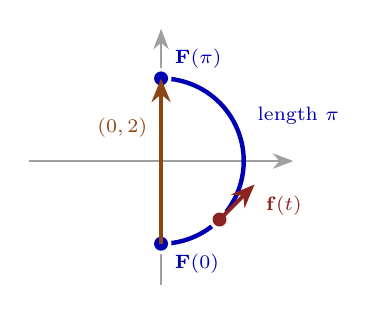
\begin{tikzpicture}[scale=1.05]
      \draw[axisln] (-1.6,0) -- (1.6,0);
      \draw[axisln] (0,-1.5) -- (0,1.6);
      % path F(t): right half of unit circle from (0,-1) to (0,1)
      \draw[curveln, blue!70!black, domain=-90:90, samples=60]
        plot ({cos(\x)}, {sin(\x)});
      \dotpt{blue!70!black}{(0,-1)}
      \dotpt{blue!70!black}{(0,1)}
      \node[blue!70!black, below right] at (0.05,-1.0) {\scriptsize $\mathbf{F}(0)$};
      \node[blue!70!black, above right] at (0.05,1.0) {\scriptsize $\mathbf{F}(\pi)$};
      \node[blue!70!black, right] at (1.05,0.55) {\scriptsize length $\pi$};
      % displacement
      \draw[vec, mAccent] (0,-1) -- (0,1);
      \node[mAccent, left] at (-0.05,0.4) {\scriptsize $(0,2)$};
      % velocity at t = pi/4
      \dotpt{thmcolor}{({cos(-45)},{sin(-45)})}
      \draw[vec, thmcolor] ({cos(-45)},{sin(-45)}) -- ({cos(-45)+0.6*cos(45)},{sin(-45)+0.6*sin(45)});
      \node[thmcolor, below right] at ({cos(-45)+0.6*cos(45)+0.02},{sin(-45)+0.6*sin(45)-0.02}) {\scriptsize $\mathbf{f}(t)$};
    \end{tikzpicture}
    \end{center}
  \end{column}
  \end{columns}

  \note{
    In the picture, the blue curve is the path traced by capital "F": it is
    the right half of the unit circle, starting at the bottom point
    capital "F" of 0 and ending at the top point capital "F" of pi. The red arrow is
    the velocity "f" at one moment, tangent to the circle and of
    length 1. The orange arrow is the displacement, the vector 0
    comma 2, which we just computed as the integral of "f". Now
    compare lengths. The orange displacement has length 2. The blue
    path has length pi, and that is the integral of the absolute
    value of "f", since the speed is constantly 1. The displacement
    2 is smaller than the distance traveled pi. That inequality
    holds in general, and proving it is our next task.
  }
\end{frame}
}

{
\usebackgroundtemplate{%
  
\includegraphics[width=\paperwidth,height=\paperheight,keepaspectratio=false]{chapter_06_bg_04.png}%
}
\section{The Triangle Inequality for Integrals}

% --- Build 1/2 ---
\begin{frame}{Why This One Needs a New Idea}
  \begin{thmblock}{Recall: Theorem 6.13(b), real case}
    If $f \in \mathscr{R}(\alpha)$, then $|f| \in \mathscr{R}(\alpha)$ and
    $\displaystyle \Big|\int_a^b f\,d\alpha\Big| \leq \int_a^b |f|\,d\alpha$.
  \end{thmblock}

  \begin{hlbox}
  \textbf{The old proof:} choose $c = \pm 1$ so that $c \int f\,d\alpha \geq 0$; then
  \[
    \Big|\int f\,d\alpha\Big| = c\int f\,d\alpha = \int cf\,d\alpha
    \leq \int |f|\,d\alpha \qquad (\text{since } cf \leq |f|).
  \]
  \end{hlbox}

  \note{
    Before the theorem, let's understand why it is not a free
    transfer. Recall part "b" of Theorem 6.13: for a real integrable
    function "f", the absolute value of "f" is integrable, and the
    absolute value of the integral is at most the integral of the
    absolute value. The proof was a sign trick. The integral of "f"
    is a real number, so we can pick "c" equal to plus or minus 1 to
    make "c" times the integral nonnegative. Then the absolute value
    of the integral equals the integral of "c" times "f", and since
    "c" times "f" is at most the absolute value of "f" pointwise,
    monotonicity finishes the job. Now watch what breaks for
    vectors.
  }
\end{frame}

% --- Build 2/2 ---
\begin{frame}{Why This One Needs a New Idea}
  \begin{thmblock}{Recall: Theorem 6.13(b), real case}
    If $f \in \mathscr{R}(\alpha)$, then $|f| \in \mathscr{R}(\alpha)$ and
    $\displaystyle \Big|\int_a^b f\,d\alpha\Big| \leq \int_a^b |f|\,d\alpha$.
  \end{thmblock}

  \begin{hlbox}
  \textbf{The old proof:} choose $c = \pm 1$ so that $c \int f\,d\alpha \geq 0$; then
  \[
    \Big|\int f\,d\alpha\Big| = c\int f\,d\alpha = \int cf\,d\alpha
    \leq \int |f|\,d\alpha \qquad (\text{since } cf \leq |f|).
  \]
  \vspace{-0.9em}

  \textbf{For vectors:}
  \begin{itemize}
    \item $\int \mathbf{f}\,d\alpha$ has \alert{no sign} --- it is a point of $R^k$
    \item $|\mathbf{f}| = (f_1^2 + \cdots + f_k^2)^{1/2}$ is \alert{not}
      built coordinate by coordinate
  \end{itemize}
  \end{hlbox}

  \note{
    Now look at what breaks for vectors. First, the integral of "f"
    is a point in "k" dimensional space; it has no sign, so there is
    no plus or minus 1 to multiply by. Second, the absolute value of
    a vector is the square root of the sum of the squares of its
    coordinates. It mixes all the coordinates together, so even the
    claim that the absolute value of "f" is integrable is not a
    coordinate by coordinate statement. Both halves of the theorem
    need a real argument. Here is the statement.
  }
\end{frame}

% --- Build 1/2 ---
\begin{frame}{Theorem 6.25: The Triangle Inequality for Integrals}
  \begin{thmblock}{Theorem 6.25}
    If $\mathbf{f}$ maps $[a, b]$ into $R^k$ and if $\mathbf{f} \in \mathscr{R}(\alpha)$
    for some monotonically increasing function $\alpha$ on $[a, b]$, then
    \[
      |\mathbf{f}| \in \mathscr{R}(\alpha).
    \]
  \end{thmblock}

  \note{
    Theorem 6.25 has two conclusions, and we take them one at a
    time. Suppose "f" maps the interval into "k" dimensional space
    and is integrable with respect to some increasing function alpha.
    The first conclusion is that the real valued function absolute
    value of "f", which assigns to each "t" the length of the vector
    "f" of "t", is also integrable with respect to alpha. That is the
    statement that makes the right hand side of the inequality
    meaningful.
  }
\end{frame}

% --- Build 2/2 ---
\begin{frame}{Theorem 6.25: The Triangle Inequality for Integrals}
  \begin{thmblock}{Theorem 6.25}
    If $\mathbf{f}$ maps $[a, b]$ into $R^k$ and if $\mathbf{f} \in \mathscr{R}(\alpha)$
    for some monotonically increasing function $\alpha$ on $[a, b]$, then
    $|\mathbf{f}| \in \mathscr{R}(\alpha)$, and
    \begin{equation}
      \left|\int_a^b \mathbf{f}\,d\alpha\right| \leq \int_a^b |\mathbf{f}|\,d\alpha. \tag{40}
    \end{equation}
  \end{thmblock}

  \vspace{0.4em}
  \begin{hlbox}
  \textbf{Why ``triangle inequality'':} for a finite sum,
  $|\mathbf{v}_1 + \cdots + \mathbf{v}_n| \leq |\mathbf{v}_1| + \cdots + |\mathbf{v}_n|$;
  \\ an integral is a limit of such sums.
  \end{hlbox}

  \note{
    The second conclusion is inequality 40: the absolute value of the
    integral of "f" is at most the integral of the absolute value of
    "f". On the left we have the length of a single vector, the
    integral; on the right we integrate the lengths. The name
    triangle inequality is apt. For finitely many vectors, the length
    of a sum is at most the sum of the lengths, by repeated use of
    the triangle inequality of Chapter 1. An integral is a limit of
    Riemann-Stieltjes sums, so inequality 40 is what the triangle
    inequality becomes in the limit. That heuristic could be made
    into a proof, but the book gives a slicker argument. Let's plan
    it.
  }
\end{frame}

\begin{frame}{Proof Strategy: Theorem 6.25}
  \begin{hlbox}
  \textbf{Part 1: $|\mathbf{f}| \in \mathscr{R}(\alpha)$.}
  \begin{itemize}
    \item $|\mathbf{f}| = \varphi(f_1^2 + \cdots + f_k^2)$ with $\varphi = \sqrt{\cdot}$
      \;$\Rightarrow$\; use the \emph{composition theorem} (6.11) twice
  \end{itemize}

  \vspace{0.5em}
  \textbf{Part 2: the inequality (40).}
  \begin{itemize}
    \item Let $\mathbf{y} = \int \mathbf{f}\,d\alpha$ be the \emph{answer}
    \item \textbf{Key trick:} measure $\mathbf{f}$ along the direction of $\mathbf{y}$:
      $\;|\mathbf{y}|^2 = \int \mathbf{y}\cdot\mathbf{f}\,d\alpha$
    \item \textbf{Schwarz:} $\mathbf{y}\cdot\mathbf{f}(t) \leq |\mathbf{y}|\,|\mathbf{f}(t)|$
      \;$\Rightarrow$\; $|\mathbf{y}|^2 \leq |\mathbf{y}| \int |\mathbf{f}|\,d\alpha$
    \item Divide by $|\mathbf{y}|$
  \end{itemize}
  \end{hlbox}

  \note{
    Here is the strategy. Part 1 handles integrability. The absolute
    value of "f" is the square root of the sum of the squares of the
    components. Squaring is continuous, the square root is continuous,
    and Theorem 6.11 says that a continuous function of an integrable
    function is integrable. So we apply that composition theorem
    twice, with linearity in between. Part 2 is the inequality, and
    here is the beautiful trick. Call the answer "y", the vector
    integral of "f". The vector "y" has no sign, but it has a
    direction. So we measure "f" along that direction by taking the
    dot product with "y". A short computation shows that the squared
    length of "y" equals the integral of the dot product of "y" with
    "f". The Schwarz inequality bounds this dot product by the
    product of the lengths, and after integrating and dividing by
    the length of "y", inequality 40 falls out. Let's execute Part 1.
  }
\end{frame}

% --- Build 1/4 ---
\begin{frame}{Proof of Theorem 6.25, Part 1: $|\mathbf{f}|$ Is Integrable}
  \begin{proofblock}{Step 1: Write $|\mathbf{f}|$ in terms of the components}
    If $f_1, \dots, f_k$ are the components of $\mathbf{f}$, then
    \begin{equation}
      |\mathbf{f}| = \big(f_1^2 + \cdots + f_k^2\big)^{1/2}. \tag{41}
    \end{equation}
  \end{proofblock}

  \note{
    Part 1 begins with formula 41, which is just the definition of
    the length of a vector in "k" dimensional space from Chapter 1:
    the absolute value of "f" of "t" is the square root of the sum
    of the squares of the coordinates "f" sub 1 of "t" through "f"
    sub "k" of "t". We will show that this function is integrable by
    building it up from the inside out: first the squares, then the
    sum, then the square root.
  }
\end{frame}

% --- Build 2/4 ---
\begin{frame}{Proof of Theorem 6.25, Part 1: $|\mathbf{f}|$ Is Integrable}
  \begin{proofblock}{Step 1: Write $|\mathbf{f}|$ in terms of the components}
    If $f_1, \dots, f_k$ are the components of $\mathbf{f}$, then
    \begin{equation}
      |\mathbf{f}| = \big(f_1^2 + \cdots + f_k^2\big)^{1/2}. \tag{41}
    \end{equation}
  \end{proofblock}

  \begin{proofblock}{Step 2: The inside is integrable}
    By Theorem 6.11 (with $\varphi(t) = t^2$), each $f_i^2 \in \mathscr{R}(\alpha)$;
    hence by Theorem 6.12(a) so does their sum
    $\;g = f_1^2 + \cdots + f_k^2 \in \mathscr{R}(\alpha)$, with $0 \leq g \leq M$.
  \end{proofblock}

  \note{
    Step 2: the expression inside the square root. Each component
    "f" sub "i" is integrable by hypothesis. Theorem 6.11 says that
    if we compose an integrable function with a continuous function
    phi, the result is integrable; taking phi of "t" equal to "t"
    squared shows that each "f" sub "i" squared is integrable. This
    is exactly how we proved that products are integrable back in
    Theorem 6.13. Then linearity, part "a" of Theorem 6.12, tells us
    that the sum of the squares, which we call "g", is integrable as
    well. The slide also records that "g" is nonnegative and bounded
    by some constant "M"; we will need that bound in the next step.
  }
\end{frame}

% --- Build 3/4 ---
\begin{frame}{Proof of Theorem 6.25, Part 1: $|\mathbf{f}|$ Is Integrable}
  \begin{proofblock}{Step 2: The inside is integrable}
    By Theorem 6.11 (with $\varphi(t) = t^2$), each $f_i^2 \in \mathscr{R}(\alpha)$;
    hence by Theorem 6.12(a) so does their sum
    $\;g = f_1^2 + \cdots + f_k^2 \in \mathscr{R}(\alpha)$, with $0 \leq g \leq M$.
  \end{proofblock}

  \begin{proofblock}{Step 3: The square root is continuous}
    $x \mapsto x^2$ is a continuous $1$--$1$ map of the compact set
    $[0, \sqrt{M}]$ onto $[0, M]$, so by Theorem 4.17 its inverse
    $\sqrt{\cdot}$ is continuous on $[0, M]$ (any $M > 0$).
  \end{proofblock}

  \note{
    Step 3: to apply the composition theorem again we need the square
    root to be continuous, and the book gets this from Theorem 4.17.
    Recall that Theorem 4.17 says a continuous one to one map from a
    compact metric space onto another metric space has a continuous
    inverse. The squaring function is continuous and one to one on
    the compact interval from 0 to the square root of "M", and it
    maps that interval onto the interval from 0 to "M". Its inverse
    is the square root, which is therefore continuous on the
    interval from 0 to "M". Since "M" was arbitrary, the square root
    is continuous wherever we need it.
  }
\end{frame}

% --- Build 4/4 ---
\begin{frame}{Proof of Theorem 6.25, Part 1: $|\mathbf{f}|$ Is Integrable}
  \begin{proofblock}{Step 2: The inside is integrable}
    By Theorem 6.11 (with $\varphi(t) = t^2$), each $f_i^2 \in \mathscr{R}(\alpha)$;
    hence by Theorem 6.12(a) so does their sum
    $\;g = f_1^2 + \cdots + f_k^2 \in \mathscr{R}(\alpha)$, with $0 \leq g \leq M$.
  \end{proofblock}

  \begin{proofblock}{Step 3: The square root is continuous}
    $x \mapsto x^2$ is a continuous $1$--$1$ map of the compact set
    $[0, \sqrt{M}]$ onto $[0, M]$, so by Theorem 4.17 its inverse
    $\sqrt{\cdot}$ is continuous on $[0, M]$ (any $M > 0$).
  \end{proofblock}

  \begin{proofblock}{Step 4: Compose once more}
    Theorem 6.11 with $\varphi = \sqrt{\cdot}$ and (41) give
    $\;\boxed{|\mathbf{f}| = \sqrt{g} \in \mathscr{R}(\alpha).}$
  \end{proofblock}

  \note{
    Step 4: now apply Theorem 6.11 once more, this time with phi
    equal to the square root, which is continuous on the range of
    "g". The composition, the square root of "g", is integrable, and
    by formula 41 that composition is exactly the absolute value of
    "f". This proves the first conclusion of the theorem. Before the
    inequality, let's look at a picture of the key trick.
  }
\end{frame}

\begin{frame}{The Key Idea: Measure $\mathbf{f}$ in the Direction of the Answer}
  \begin{center}
  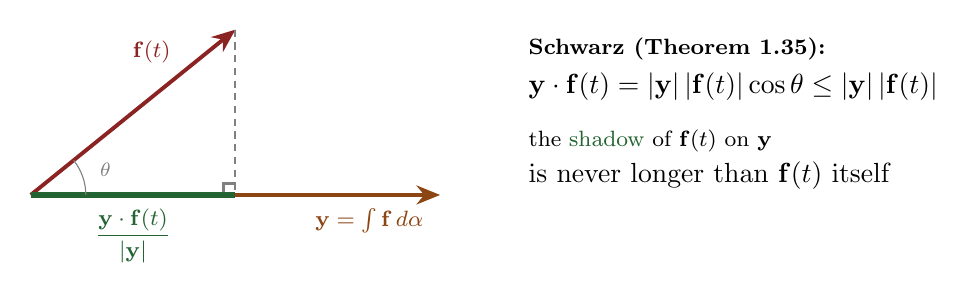
\begin{tikzpicture}[scale=1.0]
    \coordinate (O) at (0,0);
    \coordinate (Y) at (5.2,0);
    \coordinate (F) at (2.6,2.1);
    % y vector
    \draw[vec, mAccent] (O) -- (Y);
    \node[mAccent, below] at (4.3,-0.05) {\footnotesize $\mathbf{y} = \int \mathbf{f}\,d\alpha$};
    % f(t) vector
    \draw[vec, thmcolor] (O) -- (F);
    \node[thmcolor, above left] at (1.9,1.55) {\footnotesize $\mathbf{f}(t)$};
    % projection
    \draw[projln, gray] (F) -- (2.6,0);
    \draw[gray, line width=1pt] (2.45,0) -- (2.45,0.15) -- (2.6,0.15);
    \draw[line width=2.2pt, proofcolor] (O) -- (2.6,0);
    \node[proofcolor, below] at (1.3,-0.05)
      {\footnotesize $\dfrac{\mathbf{y}\cdot\mathbf{f}(t)}{|\mathbf{y}|}$};
    % angle
    \draw[gray] (0.7,0) arc (0:39:0.7);
    \node[gray] at (0.95,0.32) {\scriptsize $\theta$};
    % right side: inequality
    \node[anchor=west, align=left] at (6.2,1.6)
      {\footnotesize \textbf{Schwarz (Theorem 1.35):}\\[2pt]
       $\mathbf{y}\cdot\mathbf{f}(t) = |\mathbf{y}|\,|\mathbf{f}(t)|\cos\theta \leq |\mathbf{y}|\,|\mathbf{f}(t)|$};
    \node[anchor=west, align=left] at (6.2,0.45)
      {\footnotesize the \textcolor{proofcolor}{shadow} of $\mathbf{f}(t)$ on $\mathbf{y}$\\[1pt]
       is never longer than $\mathbf{f}(t)$ itself};
  \end{tikzpicture}
  \end{center}

  \note{
    This picture explains the trick behind Part 2. The orange arrow
    is the vector "y", the integral of "f", the answer we want to
    bound. The red arrow is the value "f" of "t" at some moment "t".
    The vector "y" has no sign, but it has a direction, and we can
    project "f" of "t" onto that direction. The green segment is the
    shadow of "f" of "t" on the line through "y"; its length is the
    dot product of "y" with "f" of "t", divided by the length of
    "y". On the right, the Schwarz inequality from Chapter 1 says
    that the dot product is at most the product of the two lengths;
    in the plane this is just the statement that the cosine of the
    angle theta is at most 1. In words: the shadow of a vector is
    never longer than the vector. We are going to integrate this
    shadow over "t" and discover that it adds up to exactly the
    length of "y". Let's do it.
  }
\end{frame}

% --- Build 1/5 ---
\begin{frame}{Proof of Theorem 6.25, Part 2: The Inequality (40)}
  \begin{proofblock}{Step 1: Name the answer}
    Put $\mathbf{y} = (y_1, \dots, y_k)$ with $y_j = \int f_j\,d\alpha$, so
    $\mathbf{y} = \int \mathbf{f}\,d\alpha$. \quad
    \textbf{Goal:} $|\mathbf{y}| \leq \int |\mathbf{f}|\,d\alpha$.
  \end{proofblock}

  \note{
    Part 2. Step 1: we give the answer a name. Let "y" sub "j" be
    the integral of component number "j", and let "y" be the vector
    with these coordinates. By Definition 6.23, "y" is exactly the
    integral of "f". Inequality 40 now reads: the length of "y" is at
    most the integral of the absolute value of "f". Notice that each
    "y" sub "j" is a fixed real number, a constant, and that is what
    the next step exploits.
  }
\end{frame}

% --- Build 2/5 ---
\begin{frame}{Proof of Theorem 6.25, Part 2: The Inequality (40)}
  \begin{proofblock}{Step 1: Name the answer}
    Put $\mathbf{y} = (y_1, \dots, y_k)$ with $y_j = \int f_j\,d\alpha$, so
    $\mathbf{y} = \int \mathbf{f}\,d\alpha$. \quad
    \textbf{Goal:} $|\mathbf{y}| \leq \int |\mathbf{f}|\,d\alpha$.
  \end{proofblock}

  \begin{proofblock}{Step 2: Express $|\mathbf{y}|^2$ as an integral (linearity, Theorem 6.12(a))}
    \[
      |\mathbf{y}|^2 = \sum_j y_j^2
      = \sum_j y_j \int f_j\,d\alpha
      = \int \Big(\sum_j y_j f_j\Big)\,d\alpha .
    \]
  \end{proofblock}

  \note{
    Step 2 is the computation at the heart of the proof. The squared
    length of "y" is the sum of the squares of its coordinates. Write
    each square as "y" sub "j" times "y" sub "j", and replace the
    second factor by its definition, the integral of "f" sub "j".
    Since "y" sub "j" is a constant, linearity pulls it inside the
    integral and then combines the "k" integrals into one. The
    integrand is the dot product of the constant vector "y" with "f"
    of "t". So the squared length of "y" is the integral of the
    shadow from the picture. Next we bound that shadow.
  }
\end{frame}

% --- Build 3/5 ---
\begin{frame}{Proof of Theorem 6.25, Part 2: The Inequality (40)}
  \begin{proofblock}{Step 2: Express $|\mathbf{y}|^2$ as an integral (linearity, Theorem 6.12(a))}
    \[
      |\mathbf{y}|^2 = \sum_j y_j^2
      = \sum_j y_j \int f_j\,d\alpha
      = \int \Big(\sum_j y_j f_j\Big)\,d\alpha .
    \]
  \end{proofblock}

  \begin{proofblock}{Step 3: Bound the integrand by the Schwarz inequality}
    \begin{equation}
      \sum_j y_j f_j(t) \leq |\mathbf{y}|\,|\mathbf{f}(t)| \qquad (a \leq t \leq b). \tag{42}
    \end{equation}
  \end{proofblock}

  \note{
    Step 3: we bound the integrand pointwise. For each fixed "t", the
    sum of "y" sub "j" times "f" sub "j" of "t" is the dot product of
    the two vectors "y" and "f" of "t" in "k" dimensional space. The
    Schwarz inequality, Theorem 1.35, says that a dot product is at
    most the product of the lengths. That is inequality 42, and it
    holds for every "t" in the interval. Geometrically it is the
    statement from the picture: the shadow of "f" of "t" on the
    direction of "y" is at most the length of "f" of "t".
  }
\end{frame}

% --- Build 4/5 ---
\begin{frame}{Proof of Theorem 6.25, Part 2: The Inequality (40)}
  \begin{proofblock}{Step 3: Bound the integrand by the Schwarz inequality}
    \begin{equation}
      \sum_j y_j f_j(t) \leq |\mathbf{y}|\,|\mathbf{f}(t)| \qquad (a \leq t \leq b). \tag{42}
    \end{equation}
  \end{proofblock}

  \begin{proofblock}{Step 4: Integrate (42) --- monotonicity, Theorem 6.12(b)}
    Both sides of (42) lie in $\mathscr{R}(\alpha)$ (Part 1 for the right side), so
    \begin{equation}
      |\mathbf{y}|^2 \leq |\mathbf{y}| \int |\mathbf{f}|\,d\alpha . \tag{43}
    \end{equation}
  \end{proofblock}

  \note{
    Step 4: we integrate inequality 42 against alpha. Part "b" of
    Theorem 6.12 says that integration preserves pointwise
    inequalities between integrable functions. The left side of 42
    is a linear combination of the components, hence integrable, and
    its integral is the squared length of "y", as we computed in
    Step 2. The right
    side is the constant length of "y" times the absolute value of
    "f", which is integrable by Part 1; here is where Part 1 pays
    off. Pulling out the constant, we get inequality 43: the squared
    length of "y" is at most the length of "y" times the integral of
    the absolute value of "f". Just one step remains.
  }
\end{frame}

% --- Build 5/5 ---
\begin{frame}{Proof of Theorem 6.25, Part 2: The Inequality (40)}
  \begin{proofblock}{Step 4: Integrate (42) --- monotonicity, Theorem 6.12(b)}
    Both sides of (42) lie in $\mathscr{R}(\alpha)$ (Part 1 for the right side), so
    \begin{equation}
      |\mathbf{y}|^2 \leq |\mathbf{y}| \int |\mathbf{f}|\,d\alpha . \tag{43}
    \end{equation}
  \end{proofblock}

  \begin{proofblock}{Step 5: Divide by $|\mathbf{y}|$}
    If $\mathbf{y} = \mathbf{0}$, (40) is trivial. If $\mathbf{y} \neq \mathbf{0}$,
    divide (43) by $|\mathbf{y}| > 0$:
    $\;\boxed{|\mathbf{y}| \leq \int |\mathbf{f}|\,d\alpha,}$ which is (40).
    \hfill $\blacksquare$
  \end{proofblock}

  \note{
    Step 5: two cases. If "y" is the zero vector, the left side of
    inequality 40 is zero and the right side is an integral of a
    nonnegative function, so 40 holds trivially. If "y" is not zero,
    its length is a positive number, and we may divide both sides of
    43 by it. What remains is that the length of "y" is at most the
    integral of the absolute value of "f", and that is inequality
    40. The proof is complete. Notice the elegance: the proof never
    needed to know the direction of "y" in advance; it simply used
    "y" itself as the measuring stick.
  }
\end{frame}

% --- Build 1/2 ---
\begin{frame}{Remarks: What Theorem 6.25 Says}
  \begin{remblock}{Geometric meaning}
    With $\mathbf{f} = \mathbf{F}'$ and $\alpha(t) = t$, Theorem 6.24 turns (40) into
    \[
      \underbrace{|\mathbf{F}(b) - \mathbf{F}(a)|}_{\text{displacement}}
      \;\leq\;
      \underbrace{\int_a^b |\mathbf{F}'(t)|\,dt}_{\text{distance traveled}} .
    \]
  \end{remblock}

  \note{
    Let's step back and read the theorem geometrically. Suppose "f"
    is the derivative of a position function capital "F", and we use the
    ordinary Riemann integral. Then Theorem 6.24 identifies the
    integral of "f" with the displacement capital "F" of "b" minus capital "F" of
    "a", and inequality 40 becomes: the length of the displacement is
    at most the integral of the speed, which is the distance
    traveled. The straight line from start to finish is never longer
    than the path actually taken. This is the picture we started the
    episode with, and in the next section the right hand side will
    be officially recognized as the length of the curve capital "F".
  }
\end{frame}

% --- Build 2/2 ---
\begin{frame}{Remarks: What Theorem 6.25 Says}
  \begin{remblock}{Geometric meaning}
    With $\mathbf{f} = \mathbf{F}'$ and $\alpha(t) = t$, Theorem 6.24 turns (40) into
    \[
      \underbrace{|\mathbf{F}(b) - \mathbf{F}(a)|}_{\text{displacement}}
      \;\leq\;
      \underbrace{\int_a^b |\mathbf{F}'(t)|\,dt}_{\text{distance traveled}} .
    \]
  \end{remblock}

  \begin{remblock}{Two more consequences}
    \begin{itemize}
      \item \textbf{Theorem 6.12(d) for vectors:}
        $|\mathbf{f}| \leq M \;\Rightarrow\; \big|\int_a^b \mathbf{f}\,d\alpha\big| \leq M[\alpha(b) - \alpha(a)]$
      \item \textbf{Theorem 5.19} (mean value inequality):
        $|\mathbf{F}(b) - \mathbf{F}(a)| \leq (b - a)\,|\mathbf{F}'(x)|$ for some $x$
        (same idea, no integral)
    \end{itemize}
  \end{remblock}

  \note{
    Two more consequences. First, we recover the missing part "d" of
    Theorem 6.12 for vectors: if the length of "f" is bounded by
    "M", then inequality 40 and monotonicity bound the length of the
    integral by "M" times alpha of "b" minus alpha of "a". So the
    only part of Theorem 6.12 with no vector version is part "b",
    monotonicity, because vectors cannot be compared. Second, compare
    Theorem 5.19, the mean value inequality from Chapter 5. It bounds
    the displacement by the length of the interval times the speed at
    some intermediate point, and its proof used the very same trick:
    dot with the displacement vector, then apply Schwarz. Same idea,
    once with a mean value and once with an integral. Let's
    summarize.
  }
\end{frame}
}

{
\usebackgroundtemplate{%
  
\includegraphics[width=\paperwidth,height=\paperheight,keepaspectratio=false]{chapter_06_bg_05.png}%
}
\section{Summary}

% --- Build 1/3 ---
\begin{frame}{Summary}
  \begin{hlbox}
  \textbf{Key takeaways from this section:}
  \begin{itemize}
    \item \textbf{Definition 6.23:} integrate \alert{componentwise};
      linearity, interval splitting, Theorems 6.17, 6.20, 6.21 all
      carry over \emph{for free}
  \end{itemize}
  \end{hlbox}

  \note{
    Let's review what we covered. First, Definition 6.23: a vector
    valued function is integrable when each component is, and its
    integral is the vector of the component integrals. Every theorem
    that can be checked one coordinate at a time transfers
    immediately: linearity, splitting the interval, linearity in the
    integrator, the reduction to the Riemann integral, and the
    smoothness of the integral as a function of its upper limit.
    Next, the Fundamental Theorem.
  }
\end{frame}

% --- Build 2/3 ---
\begin{frame}{Summary}
  \begin{hlbox}
  \textbf{Key takeaways from this section:}
  \begin{itemize}
    \item \textbf{Definition 6.23:} integrate \alert{componentwise};
      linearity, interval splitting, Theorems 6.17, 6.20, 6.21 all
      carry over \emph{for free}
    \item \textbf{Theorem 6.24 (FTC):} $\mathbf{F}' = \mathbf{f} \in \mathscr{R}$
      $\;\Longrightarrow\;$ $\int_a^b \mathbf{f}\,dt = \mathbf{F}(b) - \mathbf{F}(a)$:
      \emph{integrated velocity is displacement}
  \end{itemize}
  \end{hlbox}

  \note{
    Second, Theorem 6.24, the vector form of the Fundamental Theorem
    of Calculus. If capital "F" is an antiderivative of an integrable "f",
    the integral of "f" is capital "F" of "b" minus capital "F" of "a". Its proof
    was the template for everything that carries over: split into
    coordinates, apply the real theorem, reassemble. Physically,
    integrating the velocity over a time interval gives the net
    displacement, as we saw in the half circle example. And finally,
    the one result that needed a new idea.
  }
\end{frame}

% --- Build 3/3 ---
\begin{frame}{Summary}
  \begin{hlbox}
  \textbf{Key takeaways from this section:}
  \begin{itemize}
    \item \textbf{Definition 6.23:} integrate \alert{componentwise};
      linearity, interval splitting, Theorems 6.17, 6.20, 6.21 all
      carry over \emph{for free}
    \item \textbf{Theorem 6.24 (FTC):} $\mathbf{F}' = \mathbf{f} \in \mathscr{R}$
      $\;\Longrightarrow\;$ $\int_a^b \mathbf{f}\,dt = \mathbf{F}(b) - \mathbf{F}(a)$:
      \emph{integrated velocity is displacement}
    \item \textbf{Theorem 6.25:} $|\mathbf{f}| \in \mathscr{R}(\alpha)$ and
      $\big|\int \mathbf{f}\,d\alpha\big| \leq \int |\mathbf{f}|\,d\alpha$:
      \emph{displacement $\leq$ distance traveled};
      proof: dot with the answer $\mathbf{y}$, then \alert{Schwarz}
  \end{itemize}

  \vspace{0.4em}
  \textbf{Coming up next:} \alert{rectifiable curves} --- the length of a
  curve, and why it equals $\int_a^b |\boldsymbol{\gamma}'(t)|\,dt$.
  \end{hlbox}

  \note{
    Third, Theorem 6.25. The length of "f" is integrable, by two
    applications of the composition theorem, and the length of the
    integral is at most the integral of the length. The proof
    replaced the sign trick of the real case by a direction trick:
    dot with the answer "y", write the squared length of "y" as an
    integral, and apply the Schwarz inequality pointwise.
    Geometrically, displacement never exceeds distance traveled. In
    the next episode we make distance traveled precise: the length of
    a curve is the supremum of the lengths of inscribed polygons, and
    for a continuously differentiable curve gamma it equals the
    integral of the speed, the absolute value of gamma prime.
    Theorem 6.25 will be the key tool there. See you next time.
  }
\end{frame}
}

\end{document}
